% This is a template for use with the MSU Thesis class
% Version 3.6 2022/08/23
%
% Class options: 
%[PhD]	Doctor of Philosophy (default) 
%[DEd]	Doctor of Education
%[DMA]	Doctor of Musical Arts
%[DNP]	Doctor of Nursing Practice
%[MA]	Master of Arts
%[MS]	Master of Science
%[MAT]	Master of Arts for Teachers
%[MBA]	Master of Business Administration
%[MFA]	Master of Fine Arts
%[MIPS]	Master of International Planning Studies
%[MHRL]	Master of Human Resources and Labor Relations 
%[MMus]	Master of Music
%[MPH]	Master of Public Health
%[MPP]	Master of Public Policy
%[MSW]	Master of Social Work
%[MURP]	Master in Urban and Regional Planning 
%%
% Default is PhD
%
%
% This template has everything in the right order.
% Just add real content and you're done!
%
\documentclass[]{msu-thesis}
%
% for a prettier, but possibly non-compliant table of contents use the [mixedtoc] option
% for a plain table of contents use the [plaintoc] option
% for a horrendous looking, but possibly required table of contents, use the [boldtoc] option
%
% If you have large tables/figures that need to be in landscape mode, add the [lscape] option
%
% The class accepts 12pt, 11pt or 10pt font size options. 
% For Times New Roman as in this example document, use 12pt (default).
%
% If you require per-chapter appendices add the [chapterapp] option
%
% If you require per-chapter bibliographies add the [chapterbib] option
%
% This is standard fontenc for pdflatex
% If you use LuaLaTeX or XeLaTeX you should replace this with the fontspec package
\usepackage[T1]{fontenc}
%
% If the thesis office requires Times, we'll give them Times
% You can experiment with other font packages here if you like.
% If you are using XeLaTeX or LuaLaTeX load  TeX Gyre Termes, Times or Times New Roman font with \setmainfont
\usepackage{newtxtext,newtxmath} 
%
% Load any extra packages here
%
% You must specify the title of your thesis, your name, the field of study (not department), and the year
\title{Nonlinear Dynamics Studies at the FNAL Recycler Ring}
\author{Cristhian Gonzalez-Ortiz}
\fieldofstudy{Physics} % This should be in sentence case
\date{2024}

% If you want a dedication page, specify the text of the dedication here and uncomment the next command.
%
%\dedication{This thesis is dedicated to someone.}
%
\begin{document}

% All the stuff before your actual chapters is called the front matter
\frontmatter
% First make the title page
\maketitlepage

% if you have public abstract (optional) it should go here
%\begin{publicabstract}
% Public abstract goes here
%\end{publicabstract}

% Next make the regular abstract (obligatory)
\begin{abstract}
% Your abstract goes here.  Master's 1 page max. PhD 2 page max.
\end{abstract}

% Force a newpage
\clearpage
% Make the copyright page. The Graduate School ridiculously claims that you
% can't have a copyright page unless you pay ProQuest to register the copyright.
% This is simply not the case, so put in your copyright page whether or not you
% intend to pay Proquest to register the copyright.
% Furthermore, they have occasionally complained that the copyright mark is aligned
% to the right, even though that has been the format for more than a decade.
% If they want the copyright mark aligned to the left, use \makecopyrightpage* instead. 

\makecopyrightpage 

% If you have a dedication page, uncomment the next command to print the dedication page
%
%\makededicationpage
%
\clearpage
% Your Acknowledgements are formatted like a chapter, but with no number
\chapter*{Acknowledgements}
\DoubleSpacing % Acknowledgements should be double spaced
Your acknowledgements here.
%
\clearpage
% We need to turn single spacing back on for the contents/figures/tables lists
\SingleSpacing
\tableofcontents* % table of contents will not be listed in the TOC
%\clearpage
%\listoftables % comment this out if you have no tables
%\clearpage
%\listoffigures % comment this out if you have no figures
%
% If you have a Key to  Abbreviations/symbols you would add each abbreviation in its display order
% using as in the following examples:
\abbrev{MSU}{Michigan State University}
\abbrev{FNAL}{Fermilab National Accelerator Laboratory}
\abbrev{RR}{Recycler Ring}
\abbrev{MI}{Main Injector}
% Then issue a \clearpage and print the list 
\clearpage
\listofabbreviations 
% Comment out the code above if you have no abbreviations
% See the documentation if you need to change the width or format of the abbreviation column

% See the class documentation and the Memoir manual for how to create other lists
%
% If you are using an algorithm formatting package (e.g. algorithmicx or algorithm2e)
% please read the class documentation carefully on how to use these packages with the class
% The class provides an {algorithm} environment and a \listofalgorithms by default 
%
\mainmatter
%
% The next line removes the dots in chapter headings in the TOC
% May violate thesis office rules
%\addtocontents{toc}{\protect\renewcommand{\protect\cftchapterdotsep} {\cftnodots}}

% ALL documents using this class must have \chapter divisions
% If you are using it for an MA/MS thesis you still need to have chapters, even if they are very small.
\chapter{Introduction}
\label{sec:ch1}
 
Particle accelerators are the workhorses for modern scientific discoveries. Experimental nuclear and particle physics research benefit greatly from the progress of accelerator physics and technology. Accelerator physics is a rich field of applied physics living on the intersection of electromagnetism, solid-state and atomic physics, nonlinear mechanics, plasma physics, quantum mechanics, just to name a few \cite{sylee}. Furthermore, the design and operation of modern accelerator projects require costly enterprises of scientists, engineers, operators, and politicians coming together under one single metaphorical roof. Everyone coming together to perform \textquote{megascience} \cite{fermilab1}.         

The scientific principle of particle accelerators involves the acceleration, steering and/or storage of charged particles through electromagnetic manipulations. These manipulations occur through a plethora of devices and components that can control electromagnetic fields, e.g., magnets, electrical cavities. The group of particles that is subject to this electromagnetic handling is referred to as "the beam". The field of beam dynamics studies the interaction between the beam and the steering devices, as well as the Coulomb interactions between the beam itself---this is known as space charge physics. An additional distinction can be made when these steering devices are configured in a circular or linear fashion. This gives rise to the distinction between circular accelerators and linear accelerators (Linacs).

Furthermore, particle accelerators can be categorized by the type of elementary particles that compose the beam and how close to the speed of light they are traveling. The first category refers to the distinction between hadrons and leptons---particles that interact or do not interact through the strong force, respectively \cite{griffiths}. For example, protons and heavy ions are considered hadrons, while electrons and muons are considered leptons. The second category can be summarized if particles in the machine travel at a high or low energy. An example of a low-energy hadron machine is the heavy ion Linac at FRIB (Facility for Rare Isotope Beams) \cite{frib}. An example of a high-energy lepton machine was the Stanford Linear Accelerator located at SLAC National Accelerator Laboratory \cite{slac}. The two most famous high-energy hadron machines in history are the Tevatron \cite{tevatron}, which operated at Fermilab, and the LHC (Large Hadron Collider), operating at CERN \cite{lhc}. Furthermore, there are accelerator projects that encompass several categories such as the future EIC (Electron-Ion Collider) being built at Brookhaven National Laboratory \cite{eic}, which will use an electron ring---a lepton machine---and a heavy-ion circular accelerator---a hadron machine---to probe new physics. This is just to name a few. There's a plethora of accelerator projects around the world that are either operational, under commissioning or being designed. 

The following thesis will explore the beam dynamics of a circular machine. The research results are applied to the Fermilab Recycler Ring, which is used to store high-energy protons.

\section{Circular Accelerators and Storage Rings}

As will become more apparent on Ch. \ref{sec:ch2}, a particle accelerator can be thought of as a composition of accelerator-themed LEGO® bricks \cite{forest}. Each elemental LEGO® brick can be thought of as an accelerator component performing some mapping on the charged particles entering it. As it turns out, these LEGO® bricks can be assembled together circularly to give rise to circular accelerators. The assembly of these blocks in a particular shape gives rise to what is known as the lattice of the accelerator.

The acceleration part of these structures comes from elements inside the lattice that introduce some sort of electromotive force in the longitudinal direction. The most common example for these blocks are radio-frequency (rf) cavities \cite{sylee}, with super-conducting rf cavities also as an established technology \cite{srfcavs}. Particles that go through these elements gain energy on every pass. For the case where there are no acceleration blocks on these structures, a storage ring arises. Nevertheless, storage rings can also have rf cavities just for longitudinal beam manipulation, but no overall acceleration---such is the case of the Recycler Ring.    

Circular accelerators are special due to the fact that particles have to pass thousands or even millions of turns through the same LEGO® blocks. This gives birth to very interesting and complex dynamics inside these machines. One of these phenomena are called betatron resonances. The most simple lattice of a high energy machine is composed of focusing and steering blocks, and they are dipole and quadrupole magnets, i.e. the lowest-order multipole magnets. For reasons that will become apparent in Ch. \ref{sec:ch2}, these elements, in combination with free drift spaces, represent linear blocks. For the simplest circular machine, these linear LEGO® bricks are assembled together to create a linear lattice. A linear lattice is designed to have stable particle orbits all around the accelerator. Nevertheless, accounted or unaccounted elements, described by linear or nonlinear blocks, around the machine can perturb the stable orbits. Ultimately, the effect of these perturbations can add up coherently over many turns to push the beam out of the acceptance of the lattice, i.e., the particles hit the enclosing vacuum pipe and create beam loss. This whole process is known as a betatron resonance in a circular accelerator. A mathematical description of this process is described on Ch. \ref{sec:ch2}.

The following thesis describes an effort to mitigate the deleterious effect of these resonances in the Recycler Ring. After dipole and quadrupole, the third order of multipole magnetic fields is the sextupole component. Therefore, sextupole fields around the lattice are the source of third order betatron resonances. Specifically, this thesis explores mitigation techniques to these third order resonances, mainly in the Fermilab Recycler Ring (see Ch. \ref{sec:ch3}, Ch. \ref{sec:ch4} and Ch. \ref{sec:ch6}), but also with some experiments done at the CERN Proton Synchrotron Booster (see Ch. \ref{sec:ch5}). 

\section{Fermilab}

The best introduction to Fermilab is to cite an excerpt from Ref. \cite{fermilab1}:
\begin{displayquote}
    \begin{flushleft}
    [...] A passenger peers through the window of an airplane. As his plane flies into Chicago's O'Hare Field from the west, he notices a large ring on the ground below (see Fig. \ref{fig:fermia}). Near it he sees a towering white structure, a group of colorful smaller buildings, an expanse of forest, open fields, and lakes.

    "What is that ring?" he asks his neighbor.

    "Fermilab," she replies. "It's a physics laboratory. The government supports research there into what the universe is made of."

    "Why the ring?"

    "It's the four-mile-round main ring of a machine called the Tevatron. It turns protons into tools for looking inside the atomic nucleus. Huge magnets steer the protons around the ring, while high voltages accelerate them. [...]" (pp. 1)
    \end{flushleft}
\end{displayquote}

\begin{figure}[H]
    \centering
    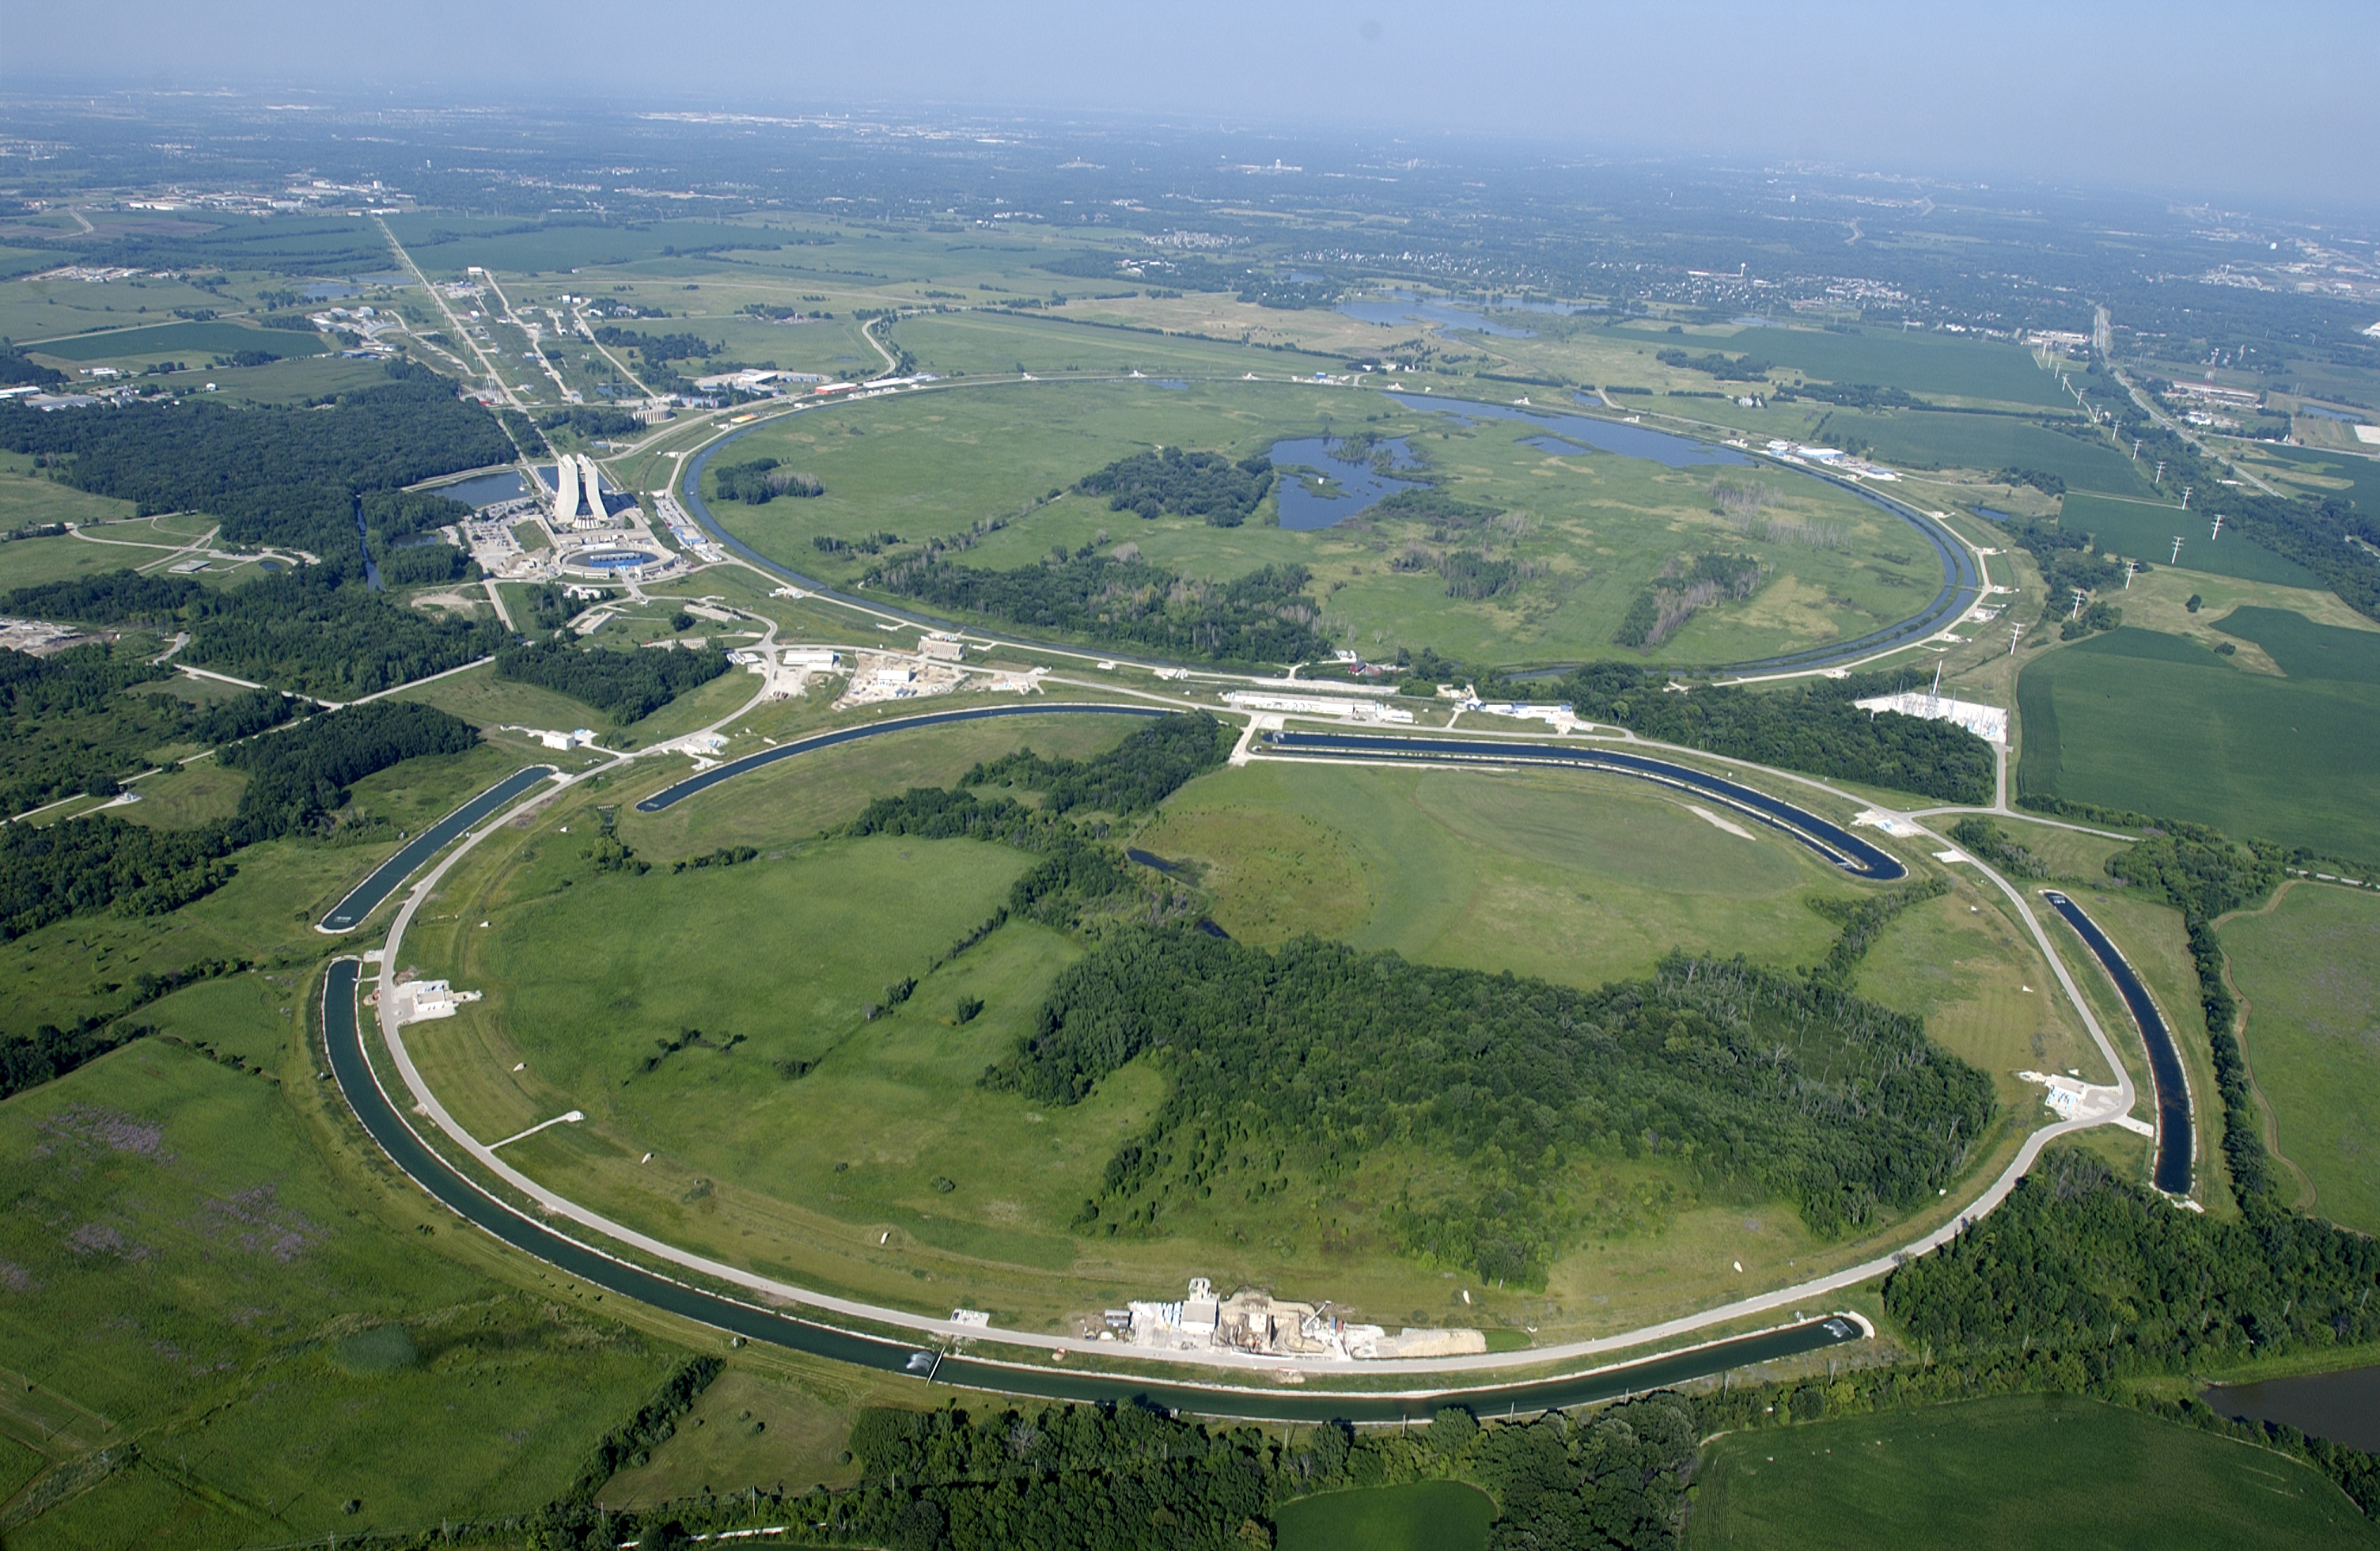
\includegraphics[width=\columnwidth]{chapter1/fermilab.jpeg}
    \caption{Aerial view of the Fermi National Accelerator Laboratory (FNAL) located in Batavia, IL, USA \cite{fermipic}.}
    \label{fig:fermia}
 \end{figure}

The Fermi National Accelerator Laboratory (FNAL), better known as Fermilab, has a long and rich history of designing, building and operating high-energy particle accelerators. Ever since the founding director of Fermilab, Robert R. Wilson, envisioned the 400 GeV Main Ring back in 1967, Fermilab has been at the forefront of accelerator physics \cite{fermilab1,fermi50,tevatron}. The most famous accelerator project hosted by Fermilab has been the Tevatron, a proton-antiproton circular collider with a circumference of around 6.28 km. This machine was injected protons and antiprotons from smaller machines, that are still in operation or have been repurposed as of 2024, e.g. the Recycler Ring. The Tevatron operated up until 2011, leaving an indelible legacy in the field of high energy and accelerator physics. Nostalgia aside, Fermilab still hosts a deluge of particle physics experiments connected to its main accelerator complex.      

The current layout of the Fermilab Accelerator Complex is summarized in Fig. \ref{fig:fac}. As of 2024, the Fermilab Accelerator Complex is composed of an $H^-$ source that connects to a linear accelerator, accelerating the ions to an energy of 400 MeV. This linear accelerator feeds to the first circular machine---the Booster---where protons are achieved and accelerated to an energy of 8 GeV. After the Booster, the protons are transported to the Recycler Ring (RR), which is the second circular machine. In the RR, protons are stacked and stored in order to increase the beam intensity delivered to the Main Injector (MI). This last circular accelerator is where protons are accelerated from an energy of 8 GeV to 120 GeV. Once at this energy, the protons are transported to the Neutrinos at the Main Injector (NuMI) experiment, in order to create the world's most intense neutrino beam \cite{numi1}. Nevertheless, all throughout the chain of accelerators, beam is also delivered to a plethora of other experiments being conducted at Fermilab. Therefore, the facility has several modes of operation depending on the experiments that are online. A more detailed and technical study of the current Fermilab Accelerator Complex, focusing on the Recycler Ring, is given on Ch. \ref{sec:ch3}.   

\begin{figure}[H]
    \centering
    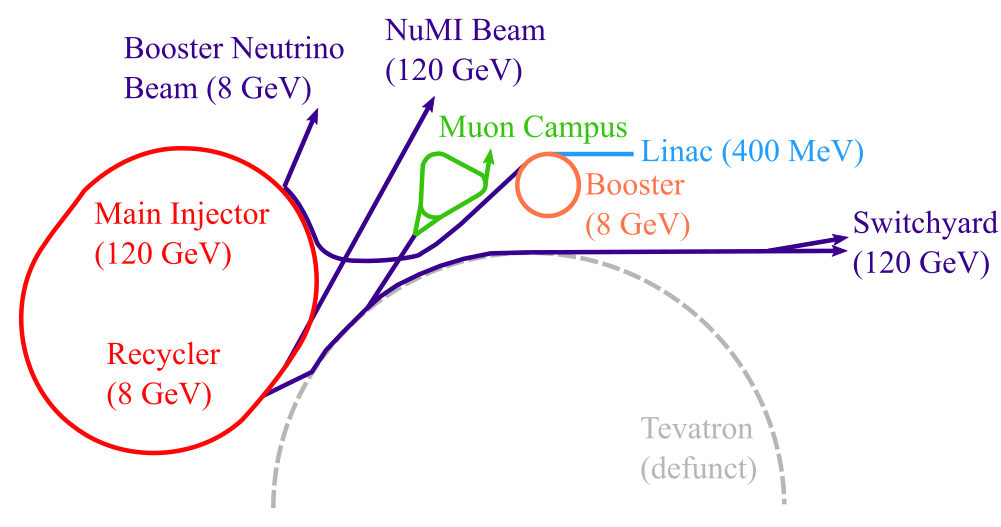
\includegraphics[width=\columnwidth]{chapter1/complex.png}
    \caption{Schematic layout of the Fermilab Accelerator Complex as of 2024. Original plot provided by R. Ainsworth, first published on Ref. \cite{rr1}.}
    \label{fig:fac}
 \end{figure}

\section{Outline}

The following thesis will explore the compensation of third-order resonances in the Fermilab Recycler Ring. \hyperref[sec:ch1]{Chapter 1} introduces the motivation behind this thesis work. \hyperref[sec:ch2]{Chapter 2} summarizes single particle dynamics with the help of exponential Lie operators and moves forward to introduce a relevant concept of collective beam dynamics: the space charge tune shift. This theoretical overview gives segue into the \hyperref[sec:ch3]{Ch. 3} of this thesis, where the Recycler Ring is introduced and described in detail. Motivation for the compensation of third order resonances is given in this chapter under the framework of current and future operation of the RR. With the basic physics concepts and the description of the machine put in place, \hyperref[sec:ch4]{Ch. 4} describes in full detail the scheme and experiments developed in order to compensate third order resonances at low intensities. Before moving to explore the Recycler Ring at high intensities, \hyperref[sec:ch5]{Ch. 5} provides an interlude in order to show a series of experiments done at the CERN PS Booster. These experiments explore the use of advanced optimization algorithms to compensate multiple resonance lines simultaneously. Coming back to Fermilab, \hyperref[sec:ch6]{Ch. 6} showcases the studies and experiments done at high intensities in the RR in order to understand the interplay between the compensation of resonance lines and space charge effects. Finally, \hyperref[sec:ch7]{Ch. 7} brings down the curtain by providing some general conclusions and future work stemming from this thesis.
\chapter{The FNAL Recycler Ring}
The Fermilab Recycler Ring (RR) is one of the circular accelerators located .

\section{General Specifications}

\section{Tune Diagram and Resonances}

\section{High Intensity and Tune Footprint}

%\chapter{Your first chapter}
%
% If you have pages that must appear in landscape mode, use the [lscape] documentclass option
% and enclose the pages in a {landscape} environment.
%\clearpage\pagestyle{lscape} % first clear the page and change the pagestyle
%\begin{landscape}
%
% your landscape table(s) or figure(s) here
%
%\end{landscape}
%\pagestyle{plain} % remember to change the pagestyle back to plain
%
%
% Your bibliography command here 
% e.g. \bibliography{your-bib-file}) if using natbib
% e.g. \printbibliography if using biblatex
%
% Remember that although the bibliography is single spaced, there needs to
% be a blank line between entries. This is set by your bibliography package
% If you are using natbib it is \bibsep; if using biblatex it's \bibitemsep
% These are set automatically by the class if you are using these packages
%
% If you need per-chapter bibliographies, you need to use the [chapterbib]
% class option and you would use \makebibliographypage before each
% chapter level bibliography and then the relevant bibliography command
% You should not use the \backmatter command 
%
% If you have appendices, they would go here.  
% If you only have one appendix it will look like this: (comment this out if you have no appendices)
\begin{appendix}
\chapter{Your appendix}
\end{appendix}
%
%
% If you have more than one appendix, you need to use 
%   \begin{appendices}
%   \chapter{First appendix}
%   \chapter{Second appendix}
%   \end{appendices}
%
% If each chapter has its own set of appendices, then load the class with the [chapterapp] option
% and put your {appendix} or {appendices} environments at the end of each chapter.
%
%
% Even though it is very unintuitive, per-chapter appendices are STILL \chapter commands
% in your document!  If you use \section it will not work properly.
% 
% You should not use the \backmatter command 
\end{document}

